\documentclass[a4 paper]{article}
%\usepackage{minted}           %embedding code
\usepackage{amsmath, amsthm, amsfonts} %always use amsmath for symbols, amsthm for theorems 
\usepackage{graphicx}  % for pictures
%\usepackage{lipsum}  % for test text
\usepackage{multicol}    % for multicollumn text
\usepackage[bottom=2.5cm]{geometry}   %to set the margins to your liking
\usepackage[skip = 10pt, indent = 30pt]{parskip}      %to set the distance between paragraphs
\usepackage{tcolorbox}           %for literal color boxes
%\usepackage{witharrows}             % understandable, arrows for equations
\usepackage{tikz}                   %drawings and diagrams
\usetikzlibrary{positioning}        %tikz library for positioning (of nodes?)
\usepackage{pgfplots}               %plotting and graphs
\pgfplotsset{compat=1.18, width = 10cm}
\usepackage{hyperref}
\hypersetup{colorlinks = true, linkcolor = black, urlcolor = blue}
%\usepackage{fancyvrb}           % fancy formatting of verbatim
%\usepackage{fancyhdr, lastpage}
%\pagestyle{fancy} 
%\lhead{Relat\'orio experimento 4}
%\rhead{FisExpI}
%\cfoot{Página \thepage \ de \pageref{LastPage}}
%\usepackage[Bjornstrup]{fncychap} %Sonny, Glenn, Lenny, Conny, Rejne, Bjarne, Bjornstrup
%\usepackage{xcolor}      %color text
\usepackage{siunitx}    %for SI units
\usepackage{setspace}
\onehalfspacing
\usepackage{cleveref}
\usepackage[brazil]{babel}
\usepackage{caption}
\usepackage{subcaption}
\usepackage{pdfpages}
\usepackage{booktabs}
\usepackage{multirow}
\usepackage{textcomp}
\usepackage{amssymb}
\usepackage[document]{ragged2e}
\usepackage{bm}





%\setlength{\hoffset}{-2cm}
%\setlength{\voffset}{1.5cm}                     %control your margins however you want!
%\setlength{\marginparwidth}{2cm}
%\setlength{\oddsidemargin}{0cm}

%\newtheorem{theorem}{Theorem}[section]               %how you call it and how you display it
%\newtheorem{corollary}{Corollary}[theorem]


\newcommand{\parag}{\hspace{30pt}}
%\newcommand{\pd}[2]{\frac{\partial#1}{\partial#2}}


\begin{document}
\justifying
\begin{center}{\large Laboratório de Circuitos Elétricos - 02/2024 - Turma 05}\\
{\large \textbf{Experimento 1}}\\ 
24/10/2024
\end{center}

\vspace{500pt}
 \noindent\textbf{Grupo 10:}\\
 Yuri Shumyatsky - 231012826


\vspace{30pt}
\newpage

\section{Introdução}
\parag O estudo de circuitos elétricos é fundamental para a compreensão dos princípios que regem o funcionamento de diversos dispositivos e sistemas eletrônicos. Neste experimento, o foco foi a utilização de equipamentos essenciais de laboratório, como a fonte de alimentação DC e o multímetro, ferramentas indispensáveis para a medição de grandezas elétricas. Além disso, o experimento visa confirmar, de forma prática, a aplicação de leis básicas dos circuitos elétricos, como as Leis de Ohm e de Kirchhoff. 

\section{Materiais}
\begin{itemize}
\item Multímetro
\item Fonte 6V
\item Protoboard
\item 2 resistores de 1,5k$\Omega$
\item 1 resistor de 1,2k$\Omega$
\end{itemize}
Montados na seguinte configuração:
\begin{table}[h]
\centering
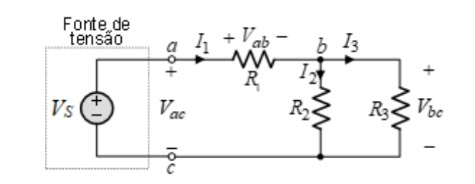
\includegraphics{figuras/circuito1}
\end{table}

\noindent Foi definido que $R_1=1,5k\Omega,\ R_2=1,2k\Omega,\ R_3=1,5k\Omega$ 

\newpage\section{Experimento}
\parag O primeiro passo é a determinação da resistência nominal de cada resistor. 

\vspace{5pt}
\begin{table}[h]
\centering
\begin{tabular}{|c|c|c|c|}
\hline
Resistor & Valor Nominal & Valor medido & Erro (\%)\\ \hline
$R_1$ & $1,5k\Omega$ & $1,4778k\Omega$ & 1,48 \\\hline
$R_2$ & $1,2k\Omega$ & $1,1832k\Omega$ & 1,4 \\\hline
$R_3$ & $1,5k\Omega$ & $1,4800k\Omega$ & 1,33 \\\hline
\end{tabular}
\caption*{Tabela 1}
\end{table}
\vspace{15pt}

\parag O segundo passo é medir as voltagens entre os pontos a e c, b e c, a e b. \\
\vspace{5pt}
\begin{table}[h]
\centering
\begin{tabular}{|c|c|c|c|}
\hline
Tensão & Valor Calculado & Valor medido & Erro (\%)\\ \hline
$V_{ac}$ &  6V & 6,0042V & 0,07 \\\hline 
$V_{ab}$ & 4,1525V & 4,1568V & 0,10\\\hline
$V_{bc}$ & 1,8475V & 1,8472V  & 0,10\\\hline
$V_{ac}-V_{ab}-V_{bc}$ & 0V &   0,0002V & - \\\hline
\end{tabular}
\caption*{Tabela 2}
\end{table}

\vspace{15pt}
\parag Com esse resultado, podemos confirmar a Lei das Tensões de Kirchhoff.

\parag Em seguida, usamos o multímetro como amperímetro para identificar as correntes.
\vspace{5pt}
\begin{table}[h]
\centering
\begin{tabular}{|c|c|c|c|}
\hline
Corrente & Valor Calculado & Valor medido & Erro (\%)\\ \hline
$I_1$ & 2,77mA & 2,8099mA & 1,47 \\\hline
$I_2$ & 1,54mA & 1,5629mA & 1,59\\\hline
$I_3$ & 1,23mA & 1,14198mA & 7,21\\\hline
$I_1-I_2-I_3$ & 0mA & 0,10502mA  & - \\\hline
\end{tabular}
\caption*{Tabela 3}
\end{table}

\newpage
\parag Em seguida verificamos a Lei de Ohm.

\begin{table}[h]
\centering
\begin{tabular}{|c|c|c|}
\hline
Corrente & Valor Calculado & Valor medido\\\hline
$V_{ab}-R_1I_1$ & 0 & 0,00432978 \\\hline
$V_{bc}-R_2I_2$ & 0 & -0,00202328 \\\hline
$V{bc}-R_3I_3$ & 0 & 0,1570696\\\hline
\end{tabular}
\caption*{Tabela 4}
\end{table}

\vspace{20pt}
\parag Esses resultados são satisfatórios para comprovar a Lei de Ohm.

\parag Após isso, é feito o cálculo das resistências equivalentes e de entrada, e as medidas com os valores experimentais.


\begin{table}[h]
\centering
\begin{tabular}{|c|c|c|c|}
\hline
Resistência & Valor Calculado & Valor medido & Erro (\%)\\ \hline
$R_{eq}$ & $0,666666667k\Omega$ & $0,65753079k\Omega$  & 1,37 \\\hline
$R_{in}$ & $2,166666667k\Omega$ & $2,13533079k\Omega$ & 1,45 \\\hline
\end{tabular}
\caption*{Tabela 5}
\end{table}

\vspace{20pt}

\parag Podemos conferir que, de fato, $\dfrac{V_{bc}}{I_1}\approx R_{eq}$ e $\dfrac{V_{ac}}{I_1}\approx R_{in}$ para os valores encontrados, sendo razoável comprovar com isso a sua igualdade.

\parag Por fim, o cálculo das potências dissipadas pelas resistências e fornecidas pela fonte, verificando com os valores teóricos.

\begin{table}[h]
\centering
\begin{tabular}{|c|c|c|c|}
\hline
Potência & Valor Calculado & Valor medido & Erro (\%)\\ \hline
Fornecida por $V_s (V_{ac}I_1)$ & 16,62mW & 16,871mW & 1,51\\\hline
Dissipada em $R_1 (V_{ab}I_1) $ & 11,51mW &   11,668mW & 1,37\\\hline
Dissipada em $R_2 (V_{bc}I_2)$ & 2,85mW & 2,890mW & 1,40\\\hline
Dissipada em $R_3 (V_{bc}I_3)$ & 2,26mW & 1,930mW & 14,98\\\hline
$P_{V_s}$ - $P_{R_1}$ -  $P_{R_2}$ - $P_{R_3}$ &   0 & 0,383 & - \\\hline
\end{tabular}
\caption*{Tabela 6}
\end{table}
\vspace{10pt}

\parag Apesar da discrepância, principalmente na medição da potência dissipada em $R_3$, que pode ser razoavelmente atribuída a falhas durante o processo de medida e/ou ao equipamento, é possível ver que $\sum P=0$.

\newpage
\section{Conclusão}
\parag Os resultados alcançados confirmaram as previsões teóricas, demonstrando a validade de leis fundamentais no estudo de circuitos elétricos, como as Leis de Kirchhoff, de Ohm, etc.  Além disso, a potência fornecida pela fonte de tensão correspondeu à soma das potências dissipadas nos resistores, comprovando a conservação da energia elétrica no circuito. 


\end{document}